% !TeX root = main.tex
% !TeX spellcheck = en_US

\documentclass[aspectratio=169,9pt]{beamer}

\usepackage{royslides}
\usepackage{graphicx}     % More options for \includegraphics
\usepackage{subfig}
\graphicspath{{figures/}} % Setting the graphicspath




\title{Quantum advantage using high-dimensional twisted photons as quantum finite automata}
\date{Milan University, 2022}
\author{Roy Stegeman}
\institute{University of Milan and INFN Milan}


% The "twisting" of a photon is done by introducing orbatial angular momentum (OAM). See: https://opg.optica.org/optica/fulltext.cfm?uri=optica-5-6-682&id=389941
% Structured photons are photons with well-engineerd polarizationa nd spatial and temporal modes. See:  https://onlinelibrary.wiley.com/doi/abs/10.1002/9781119662945.ch14
% In this case structured refers to the fact that we control the LG modes


\begin{document}
% TITLEPAGE ====================================================================
{
\setbeamertemplate{headline}{} % remove headline from titlepage
\begin{frame}
  \titlepage


  Based on arXiv:2202.04915

\end{frame}
}


% INTRO ========================================================================

\begin{frame}[t]{Content}
  \textit{Quantum advantage using high-dimensional twisted photons as quantum finite automata}
  \vspace*{1em}
  \begin{itemize}
    \item What are quantum finite automata (QFA)?
    \item Photons as qubits
    \item Experimental setup
    \item Results
  \end{itemize}
  \vspace*{5em}
  Unless otherwise specified, figures are taken from:
  \begin{itemize}
    \item arXiv: 2202.04915
    \item ``Multi-Qubit Quantum Finite
    Automata Using Structured
    Photons'', 2021, Thesis, S. Plachta
  \end{itemize}
\end{frame}


% QUANTUM FINITE AUTOMATA ======================================================
\section{Quantum Finite Automata (QFA)}
\begin{frame}[t]{Finite State Automaton}
  \begin{itemize}
    \item Abstract machine that can be in one of a finite number of states at a given time
    \item Binary decision (yes or no)
    \item Computational model simpler than a Turing machine
    \item FSA is fully defined by initial state, list of states and inputs that trigger each transition
    % \item Memory of a FSA is represented by the finite number of states in which a FSA can be
    \item FSA can be deterministic or probabilistic (a QFA is probabilistic)
  \end{itemize}
  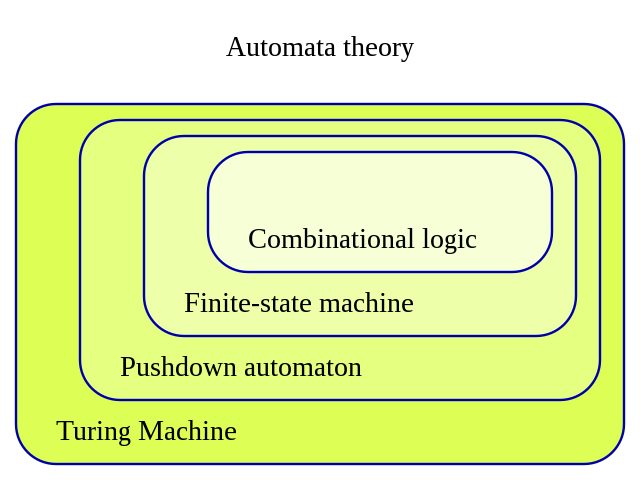
\includegraphics[width=0.35\textwidth]{Automata_hierarchy.png}
  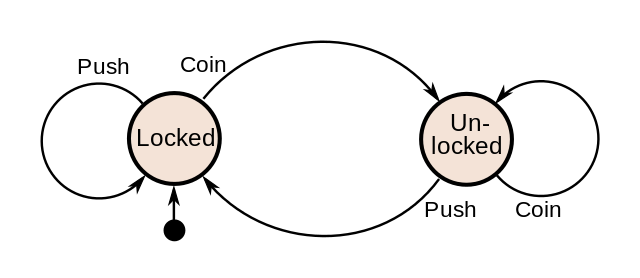
\includegraphics[width=0.4\textwidth]{turnstile.png}
\end{frame}


\begin{frame}[t]{Deterministic Finite Automata for $MOD_p$}
  \begin{itemize}
    \item This talk: is the input string a multiple of prime number $p$?
    \item Formal language: sequence of words should comply with rules (mathematical or grammar)
    \item Language is $MOD_p=\{a^n|n \mod(p)\equiv 0\}$  
    %  recognizing $MOD_n=\{a^j|j \mod n \equiv 0 \}$ for $n>1$
    % \item Decision problem: is the length of an input string a multiple of $n$?
    % \item See the representation of our $MOD_n$ problem (only accepting state is $s_0$):\\
    % \item For each symbol $a$, the DFA performs a transition between the states
    % \item If the length is a multiple of $n$, the system transitions back to its initial (and only accepting) state.
    \item \textbf{There is no deterministic FA with less than $p$ states for $MOD_p$}
  \end{itemize}
  \vspace*{2em}
  \begin{figure}
    \centering
      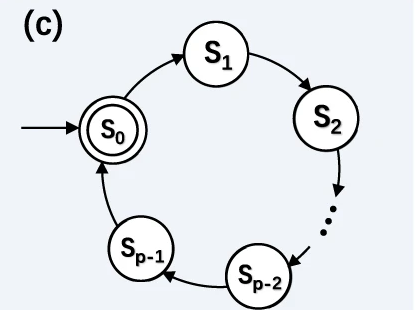
\includegraphics[width=0.3\textwidth]{QFA_MODn.png}\\
      \caption*{Schematic representation of the $MOD_p$ language}
  \end{figure}
\end{frame}


\begin{frame}[t]{Quantum Finite Automaton}
  \begin{itemize}
    % \item QFA are a special case of PFA
    \item Can make more than one transition with probabilities that sum to one
    \item Probablity of accepting is the sum of probablities corresponding to the accepting states
    \item QFA algorithm for $MOD_p$ can be more time and memory efficient than classical methods
    % \item The input $x=x[1] x[2] \cdots x[l]$ can be traced linearly
    % \item at any step an $m$-state PFA is in a probability distribution of its states represented by $v=\left(\begin{array}{llll}p_{1} & p_{2} & \cdots & p_{m}\end{array}\right)^{T}$
    % \item transformation: $v_{f}=A_{\$} A_{x[l]} A_{x[l-1]} \cdots A_{x[1]} A_{\mathbb{C}} v_{0}$
  \end{itemize}
  \begin{figure}
    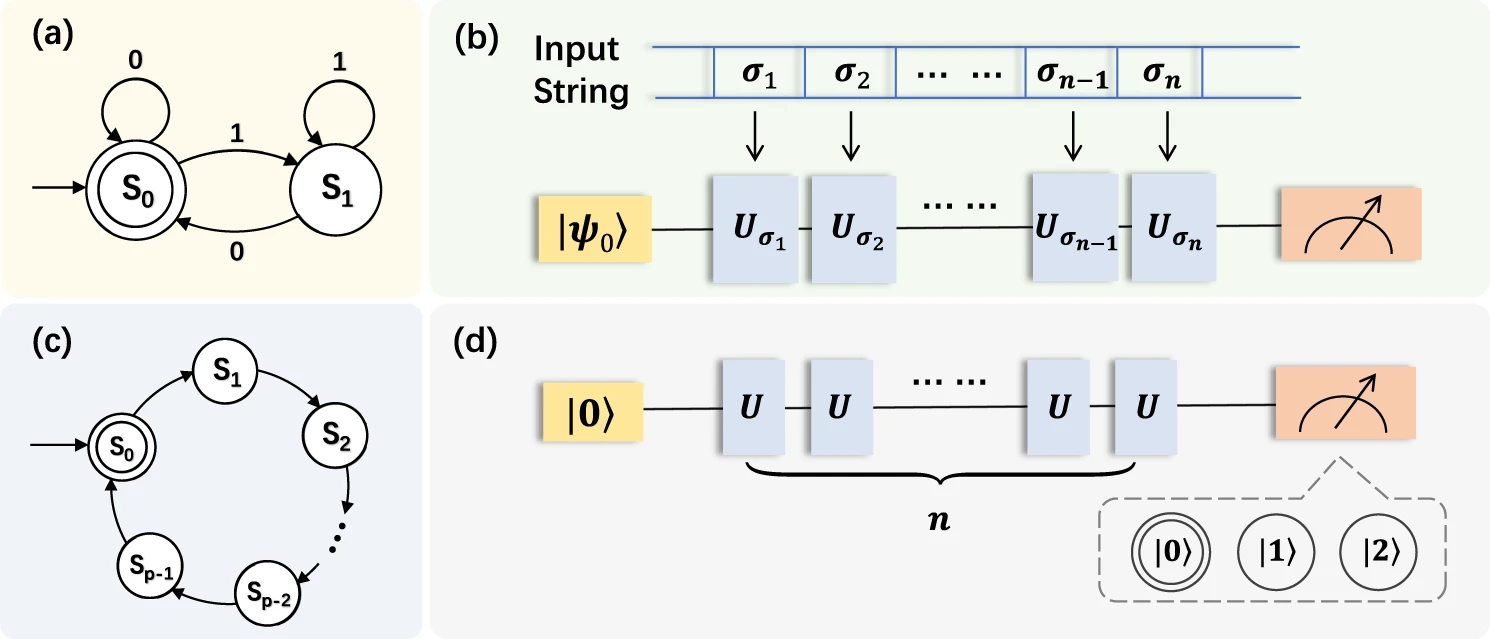
\includegraphics[width=0.6\textwidth]{DFA.png}
    \caption*{image: npj Quantum information 5, 56 (2019)}
  \end{figure}
\end{frame}


% \begin{frame}[t]{Quantum Finite Automata}
%   \begin{itemize}
%     \item Quantum counter part of PFA
%     \item QFA alorithm for MODp is one of the first quantum alogirhtms with exponental advantage over classical methods
%     \item QFA with $m$ basis states: $N=\left\{\left|q_{1}\right\rangle, \ldots,\left|q_{m}\right\rangle\right\}$
%     \item $\left|v_{f}\right\rangle=U_{\$} U_{x[l]} U_{x[l-1]} \cdots U_{x[1]} U_{\mathbb{C}}\left|v_{0}\right\rangle$
%     \item $\sum_{q_{j} \in N_{a}}\left|\left\langle q_{j} \mid v_{f}\right\rangle\right|^{2}$, $N_a$ are the accepting states
%     \item \textbf{Very similar to PFA but exponentially smaller than any classical (even randomized) FA (Ambainis and Freivalds, 1998)}
%   \end{itemize}
% \end{frame}


% \begin{frame}[t]{2-state QFA}
%   \begin{itemize}
%     \item Two basis states: $|0\rangle,|1\rangle$ ($|0\rangle$ is the accepting state)
%     % \item Identity applied when reading $\$,\mathbb{C}$ 
%     \item Input $x=a^n$, each a rotates by $\theta=2\pi/p$, thus reading of $a$
%     leads to $U_{a}=\left(\begin{array}{rr}\cos \theta & -\sin \theta \\ \sin \theta & \cos \theta\end{array}\right)$
%     \item thus the final state is $\left|v_{f}\right\rangle=\left(\begin{array}{c}\cos n \theta \\ \sin n \theta\end{array}\right)$
%     \item Input accepted with $\cos^2(2n\pi/p)$, so 1 if $n=p$
%     \item False acceptance rate up to $\cos^2(\pi/p)$
%     \item 2d-state QFA reduced false acceptance rate of 2-state QFA
%     \item Different acceptance rate for differnet $k$ run in parallel
%     \item Eq. (14)
%   \end{itemize}
% \end{frame}



% QFA using photons ===========================================================
\section{Photons as qubits}

\begin{frame}[t]{Photon beam}
  \begin{columns}[T]
    \begin{column}[]{0.45\textwidth}
      \begin{itemize}
        \item Performing the calculation on a quantum computer bacame random after reading a few symbols due to relatively large noise
        \vspace*{1em}
        \item Photon beam described by paraxial wave equation $\left(\Delta_\perp^2+2ik\frac{\partial}{\partial z}\right)u=0$
        \item Special propagation property: described by radial $p$ and azimuthal $l$ quantum numbers
        \item Laguerre-Gaussian modes $L^p_l$ as lab realization of quantum states
        % \item all modes are orthoganol
        % \item the modes have high-dimensional states (infintely many)
        % \item used to encode single photons with quantum states
      \end{itemize}
    \end{column}
    \begin{column}[]{0.05\textwidth}
    \end{column}
    \begin{column}[]{0.45\textwidth}
      \vspace*{-5em}
      \begin{figure}
        \subfloat[\centering $l=1$, $p=0$]{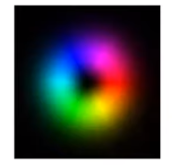
\includegraphics[width=0.4\textwidth]{l_1_p_0.png}}
        \subfloat[\centering $l=-1$, $p=0$]{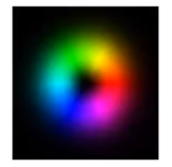
\includegraphics[width=0.4\textwidth]{l_-1_p_0.png}}
      \end{figure}
      \begin{figure}
        \subfloat[\centering $l=4$, $p=0$]{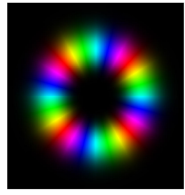
\includegraphics[width=0.4\textwidth]{l_4_p_0.png}}
        \subfloat[\centering $l=-1$, $p=2$]{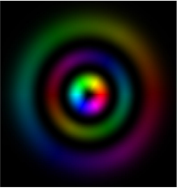
\includegraphics[width=0.4\textwidth]{l_-1_p_2.png}}
      \end{figure}
    \end{column}
  \end{columns}
\end{frame}


\begin{frame}[t]{Photonic qubits}
  \begin{columns}
    \begin{column}[]{0.5\textwidth}
      \begin{itemize}
        \item physical realization of a qubit
        \item block sphere analogue with LG modes: $|\psi\rangle=\cos(\theta/2)|L_1\rangle + e^{i\phi}\sin(\theta/2)|L_{-1}\rangle$
        \item choise of basis states: \\
        $|0\rangle= \frac{1}{\sqrt{2}}(|L_1\rangle + |L_{-1}\rangle)$\\
        $|1\rangle= \frac{1}{\sqrt{2}}(|L_1\rangle - |L_{-1}\rangle)$
      \end{itemize}
      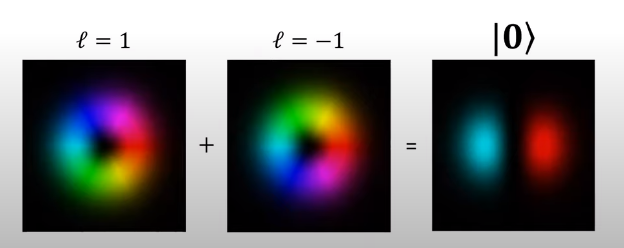
\includegraphics[width=0.99\textwidth]{photonic_superposition_qubit.png}
    \end{column}
    \begin{column}[]{0.5\textwidth}
      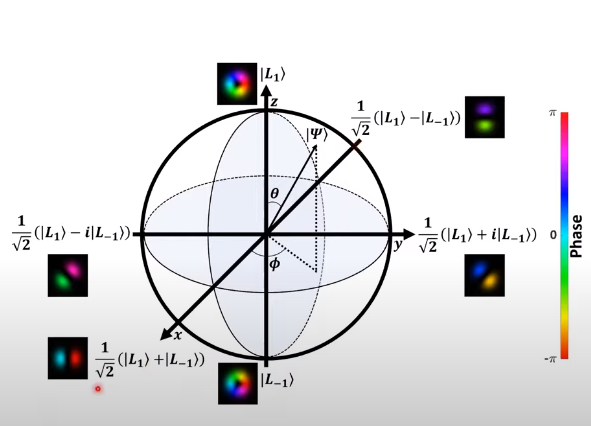
\includegraphics[width=0.99\textwidth]{photonic_bloch_sphere.png}
    \end{column}
  \end{columns}
\end{frame}

\begin{frame}[t]{Photonic qubits}
  % Superposition correpond to the multiple 2-steate QFA of the theory part(?)\\
  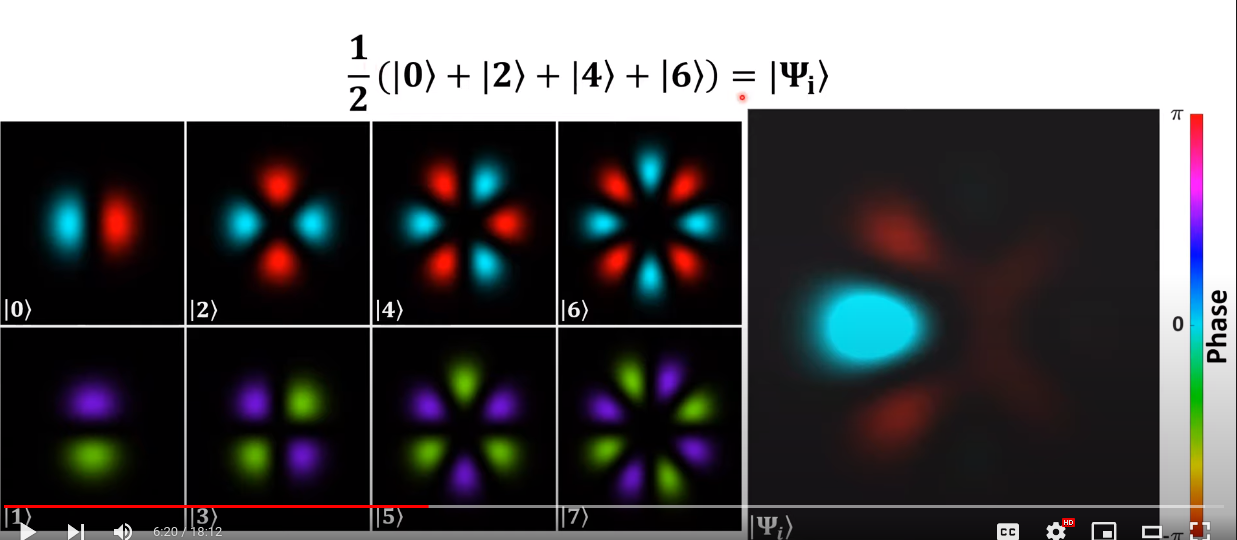
\includegraphics[width=0.5\textwidth]{4photon_qubit_superposition.png}
  \begin{itemize}
    \item $|0\rangle= \frac{1}{\sqrt{2}}(|L_1\rangle + |L_{-1}\rangle)$
    \item $|1\rangle= \frac{1}{\sqrt{2}}(|L_1\rangle - |L_{-1}\rangle)$
    \item $|2\rangle= \frac{1}{\sqrt{2}}(|L_2\rangle + |L_{-2}\rangle)$
    \item $|3\rangle= \frac{1}{\sqrt{2}}(|L_2\rangle - |L_{-2}\rangle)$
    \item \ldots
  \end{itemize}
  $|\psi\rangle = \frac{1}{{2}}(|0\rangle+|2\rangle+|4\rangle+|6\rangle)$\\
\end{frame}


% EXPERIMENTAL SETUP ===========================================================
\section{Experimental Setup}
\begin{frame}[t]{Experimental setup}
  Rephrase problem: \textit{do $n$ identical operations return the systm to its initial state?}
  \begin{columns}[T]
    \begin{column}{0.4\textwidth}
      \begin{itemize}
        \item Single photons
        \item Detector 1 \& time tagger
        \item Spatial Light Modulator (SLM)
        \item 50:50 Beam Splitter (BS)
        \item Dove prism performs the rotation operation
      \end{itemize}
    \end{column}
    \begin{column}{0.6\textwidth}
      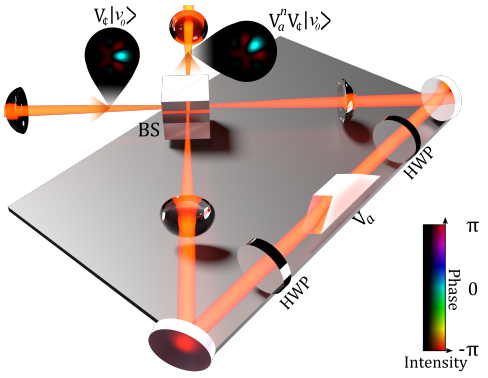
\includegraphics[width=0.8\textwidth]{experimental_setup.png}\\
    \end{column}
  \end{columns}
  % Remember eq(14)
\end{frame}


\begin{frame}[t]{Measurement}
  \begin{columns}[T]
    \begin{column}{0.4\textwidth}
      \begin{itemize}
        \item Decay as result of 50:50 beamsplitter
        % \item Principle used for prime number search
        \item Example: prime number 5
      \end{itemize}
      \vspace*{1em}
      \only<2>{\textbf{Peaks don't compeltely vanish for $n\neq5$!}}
    \end{column}
    \begin{column}{0.6\textwidth}
      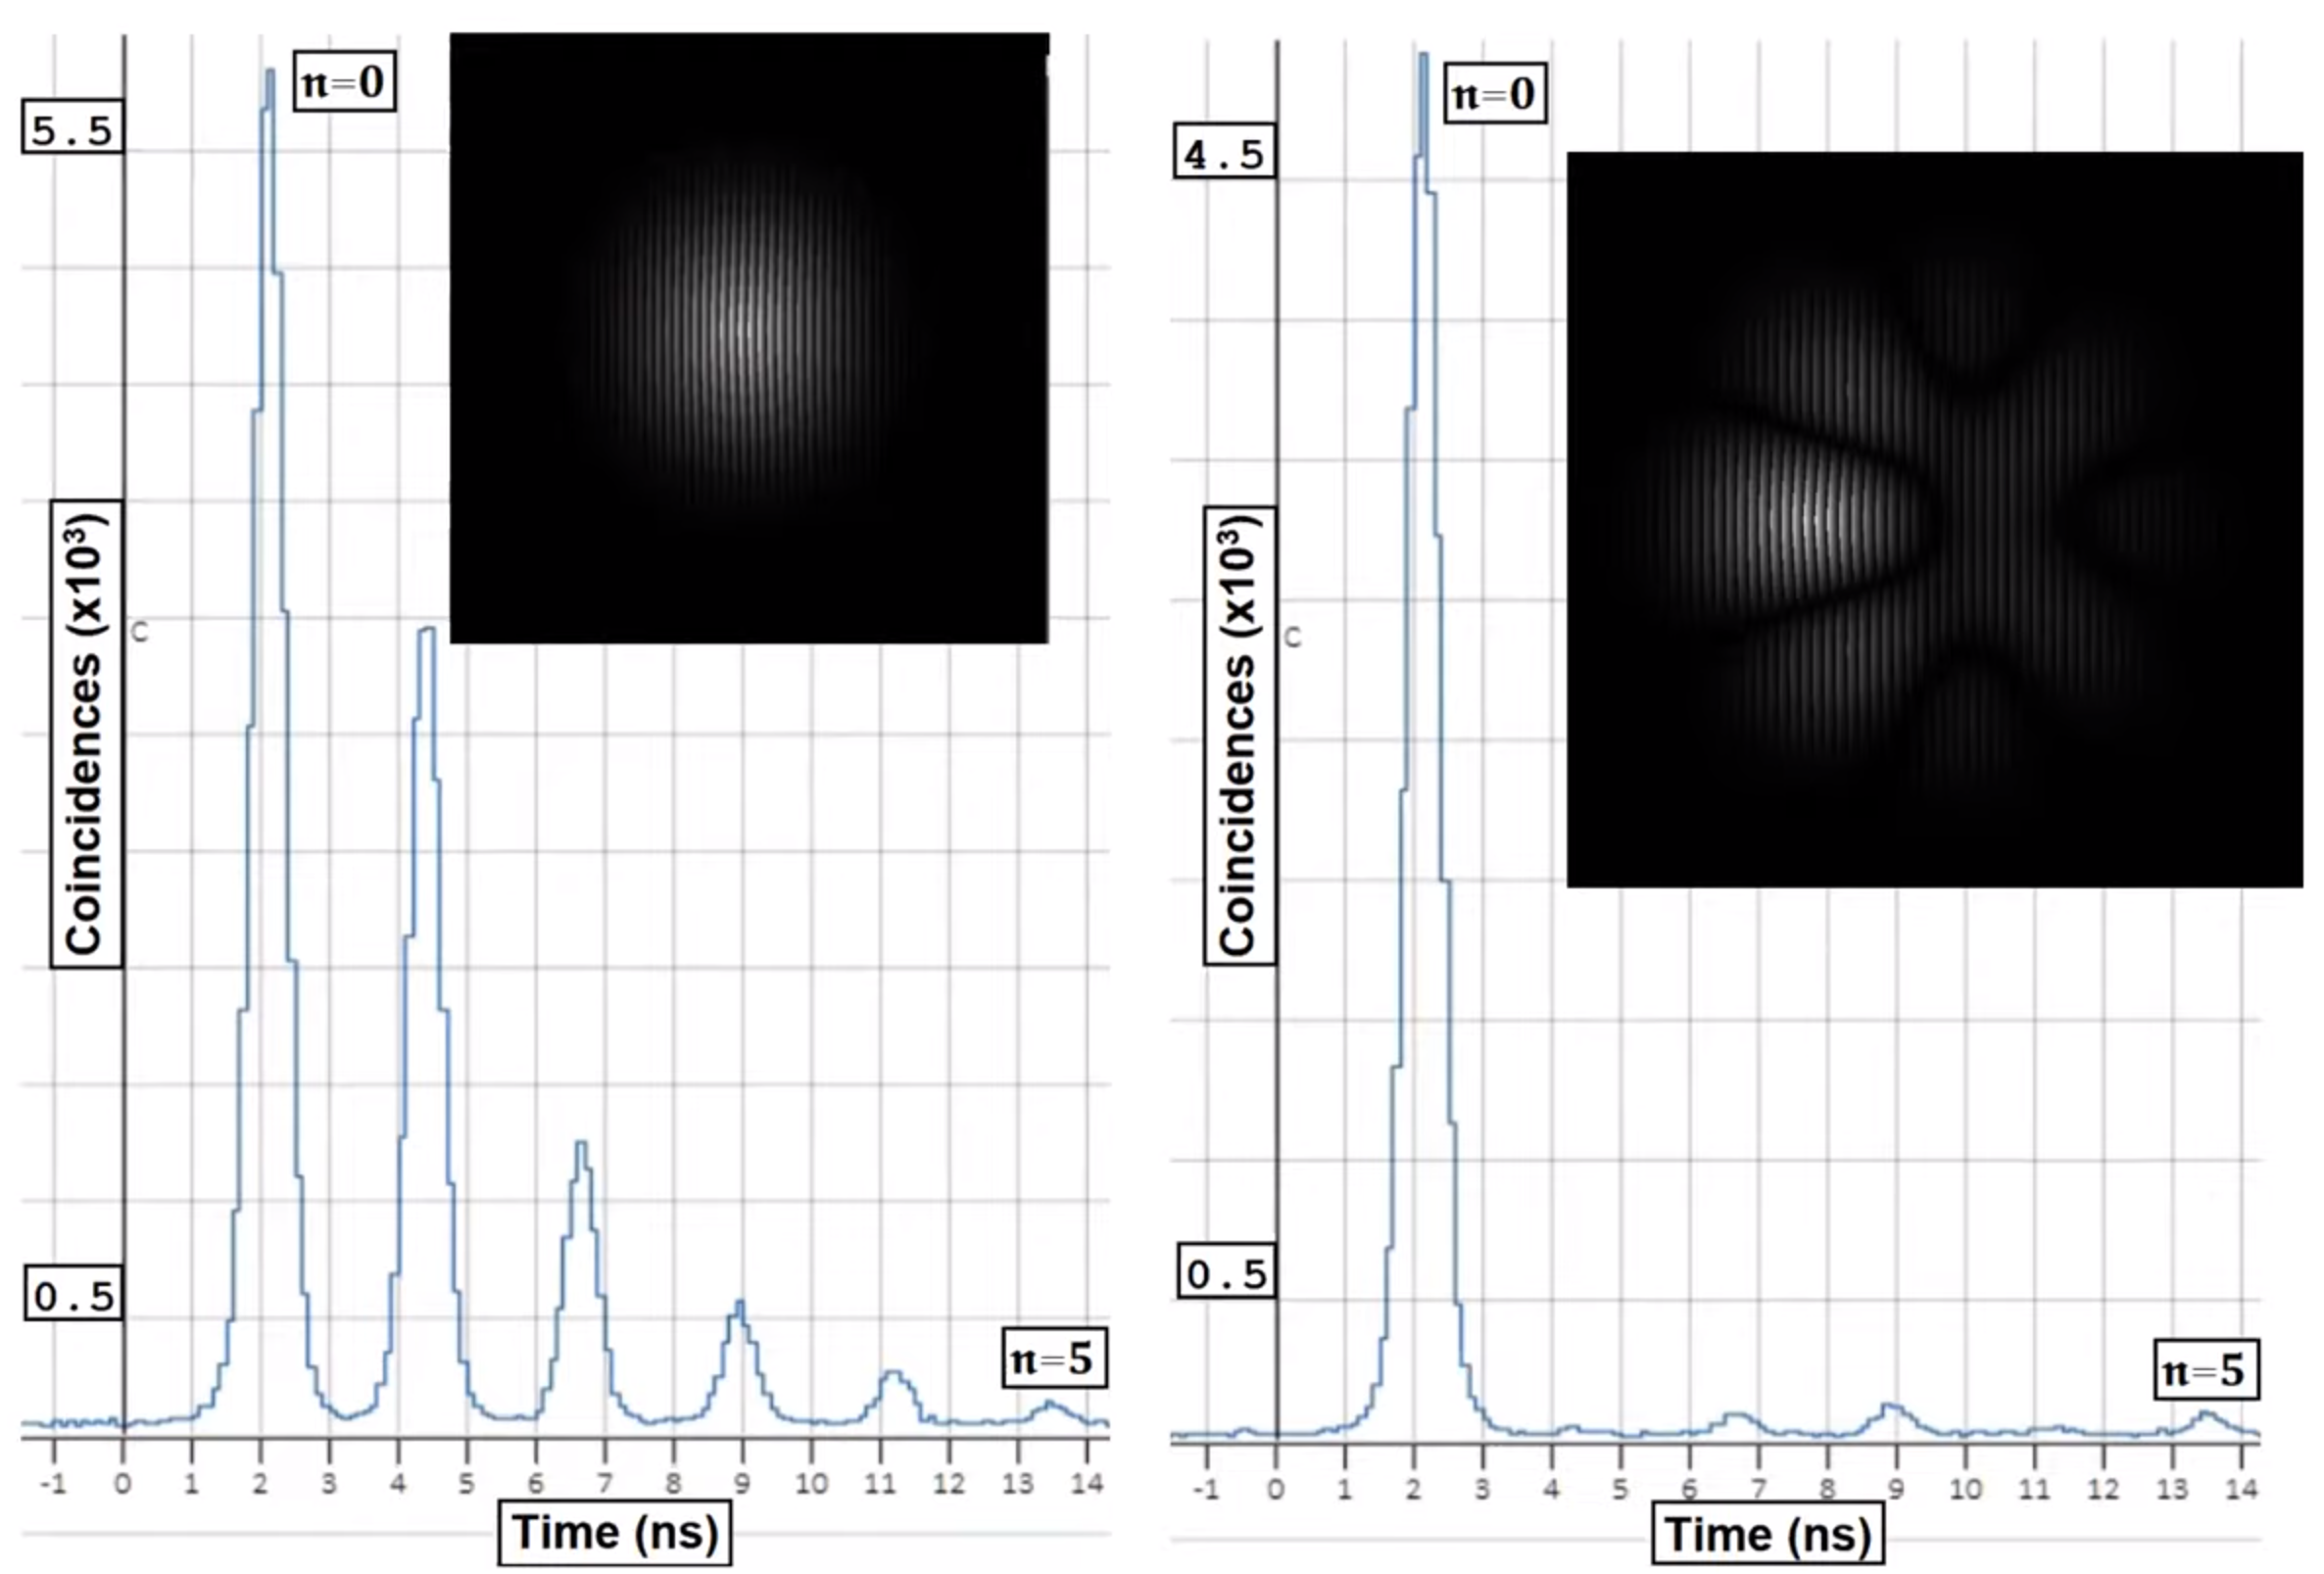
\includegraphics[width=0.9\textwidth]{example_measurement.png}
    \end{column}
  \end{columns}
\end{frame}



\begin{frame}[t]{Acceptance rate}
  \begin{itemize}
    \item Consider two basis states: $|0\rangle,|1\rangle$ ($|0\rangle$ is the accepting state)
    % \item Identity applied when reading $\$,\mathbb{C}$
    \item Input string of $n$ symbols, 
    \item each symbol rotates by $\theta=2\pi/p \Rightarrow U_{a}=\left(\begin{array}{rr}\cos \theta & -\sin \theta \\ \sin \theta & \cos \theta\end{array}\right)$
    \item thus the final state is $\left|v_{f}\right\rangle=\left(\begin{array}{c}\cos n \theta \\ \sin n \theta\end{array}\right)$
    \item Input accepted with $\cos^2(2n\pi/p)$, so probability is 1 if $n$ is multiple of prime number $p$
    \item False acceptance if $n$ is not a multiple of $p$
    \item multiple-state QFA reduces false acceptance rate of 2-state QFA
    % \item Different acceptance rate for differnet $k$ run in parallel
    % \item Eq. (14)
    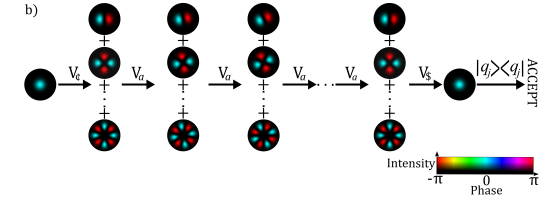
\includegraphics[width=0.6\textwidth]{2dstate.png}
  \end{itemize}
\end{frame}


% RESULTS ======================================================================
\section{Results}
\begin{frame}[t]{Recognizing $MOD_5$}
  \begin{columns}
    \begin{column}{0.5\textwidth}
      2 states: $l=1$\\
      4 states: $l=\{0,3\}$\\
      Dove prism rotates by $36^{\circ}$ \\
      $5 \times 36^{\circ} = 180^{\circ}$ (global phase symmetry)
      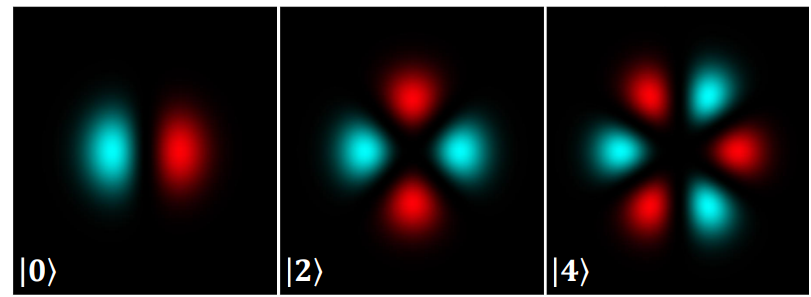
\includegraphics[width=0.9\textwidth]{multi_qbit_photon_states.png}
    \end{column}
    \begin{column}{0.5\textwidth}
      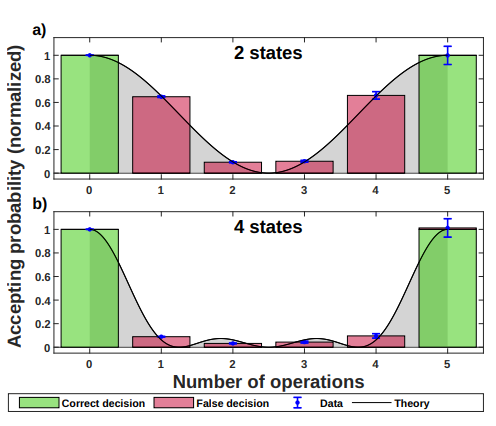
\includegraphics[width=0.9\textwidth]{2states_4states.png}
    \end{column}
  \end{columns}
  \begin{itemize}
    \item 2 states result in a high false acceptance rate
    \item 4 states gives good results (as opposed to 5 for classical)
  \end{itemize}
\end{frame}


\begin{frame}[t]{Recognizing $MOD_{11}$}
  \begin{itemize}
    \item 70:30 beam splitter to increase the number of loops
  \end{itemize}
  \begin{center}
    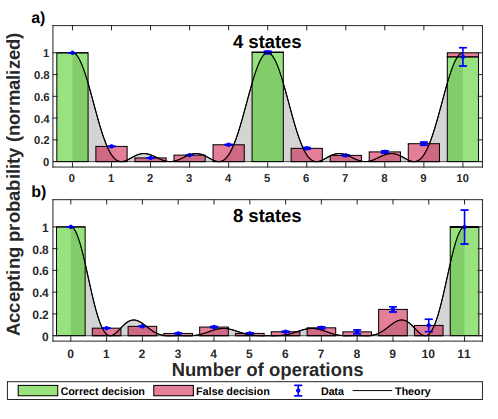
\includegraphics[width=0.4\textwidth]{4states_8states.png}\\
    % \only<2>{\Large \textbf{Thank you!}}
  \end{center}
\end{frame}


% \begin{frame}[t]{Summary}
%   \begin{itemize}
%     \item Photonic realization of QFA
%     \item Structured photons as multi-qubit states
%     \item Demonstrates efficiency with 2-qubit QFA compared to classical FA (4 instead of 5 states / 8 instead of 11 states)
%   \end{itemize}
% \end{frame}


{ % to remove the header for this frame
\makeatletter % to change template
    \setbeamertemplate{headline}[default] % not mandatory, but I though it was better to set it blank
    \def\beamer@entrycode{\vspace*{-\headheight}} % here is the part we are interested in :)
\makeatother
\begin{frame}
  \begin{center}
    \textbf{\Large Thank you!}
  \end{center}
\end{frame}
}





\begin{frame}{Determination of the photon PDF}
  \begin{columns}[T]
    \begin{column}{0.59\textwidth}
      Initially the photon PDF has been determined in different ways:
      \begin{itemize}
        \item physical model: sensitive to underlying model
        \item fitting: data does not provide strong constraints
      \end{itemize}

      \vspace*{0.5em}
      However with the LUXqed approach it can be computed perturbatively \\
      based on the observation that the heavy-lepton production cross-section can be written in two ways:
      \begin{itemize}
        \item in terms of structure functions $F_2$, $F_L$
        \item in terms of PDFs (including the photon)
      \end{itemize}

      \vspace*{0.5em}
      luxQED result {\color{gray}\small[Manohar, Nason, Salam, Zanderighi: 1607.04266, 1708.01256]}:
      \vspace*{-0.8em}
      \begin{equation*}
        \begin{split}
          & x \gamma(x, \mu^2)
          =
          \frac{2}{\alpha (\mu^2)} \int\limits_x^1 \frac{dz}{z}
          \Biggl\{ \int_{m_p^2x^2 \over 1-z}^{\mu^2 \over 1-z} \frac{dQ^2}{Q^2}
          \alpha^2(Q^2) \Biggl[ -z^2 F_L(x/z, Q^2) \\
          & + \left( z P_{\gamma q}(z) + \frac{2 x^2 m_p^2}{Q^2} \right)
          F_2(x/z, Q^2)\Biggr] - \alpha^2(\mu^2) z^2 F_2(x/z, \mu^2)\Biggr\}
        \end{split}
      \end{equation*}
    \end{column}

    \begin{column}{0.39\textwidth}
      \vspace*{-2.5em}
      \begin{figure}
        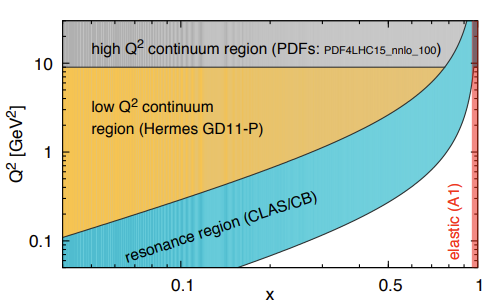
\includegraphics[width=0.89\textwidth]{figures/dataluxqed.png}
        \caption*{Input to construct $F_2$ and $F_L$}
        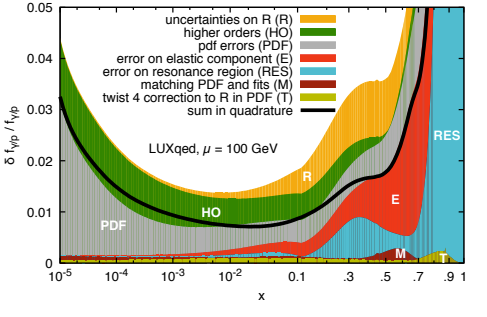
\includegraphics[width=0.89\textwidth]{figures/luxQED_uncs.png}
        \caption*{Sources of uncertainty}
      \end{figure}
    \end{column}
  \end{columns}
\end{frame}


\begin{frame}{LUXqed PDF determinations}
  LUXqed has been used in all of the most recent QED PDFs:
  \begin{itemize}
      \item LUXqed\_plus\_PDF4LHC15 {\color{gray}\small [1607.04266]}
      \item LUXqed17\_plus\_PDF4LHC15 {\color{gray}\small [1708.01256]}
      \item MMHT2015qed {\color{gray}\small [1907.02750]}
      \item NNPDF3.1luxQED {\color{gray}\small [1712.07053]}
      \item CT18lux and CT18qed {\color{gray}\small [2106.10299]}
      \item MSHT20QED {\color{gray}\small [2111.05357]}
      \item MSHT20qed\_an3lo {\color{gray}\small [2312.07665]}
      \item NNPDF4.0QED {\color{gray}\small [2401.08749 ]}
  \end{itemize}
\end{frame}

% \begin{frame}{Results: photon PDF and luminosity}
%   \begin{center}
%     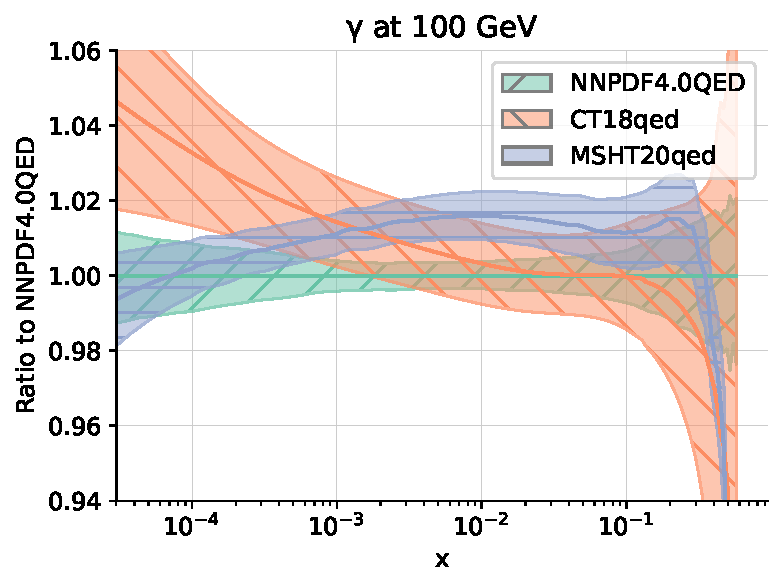
\includegraphics[width=0.3\textwidth]{figures/photon_comparison.pdf}
%     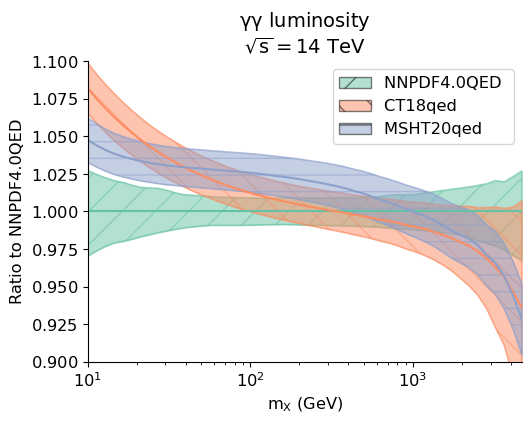
\includegraphics[width=0.3\textwidth]{figures/pp_lumi_comparison.png}
%     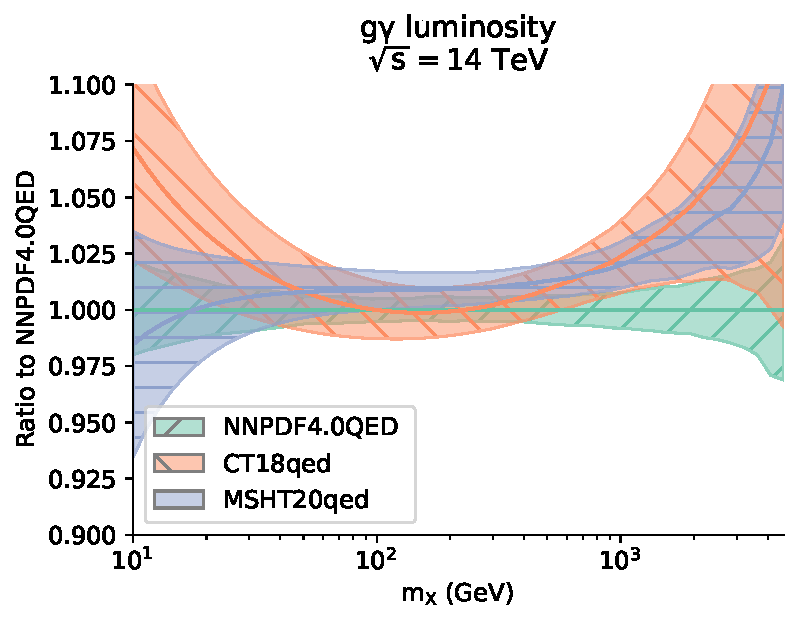
\includegraphics[width=0.3\textwidth]{figures/gp_lumi_comparison.pdf}
%   \end{center}
%   \begin{itemize}
%     \item Because all groups use the luxQED formalism, the photon PDFs agree at percent level
%     \item Luminosity generally in agreement, but differ at very small and very large invariant mass
%   \end{itemize}
% \end{frame}


% ============================================================================


\begin{frame}{Incomplete higher order uncertainties covmat}
  \begin{itemize}
    \item We construct an IHOU matrix following a similar approach by varying the subleading functions
    \item IHOU are independent of MHOU so the uncertainties are added in quadrature
    $$C = C_\mathrm{exp}+C_\mathrm{MHOU}+C_\mathrm{IHOU}$$
  \end{itemize}

  \begin{columns}
    \begin{column}{0.49\textwidth}
      \begin{figure}[!t]
        \centering
        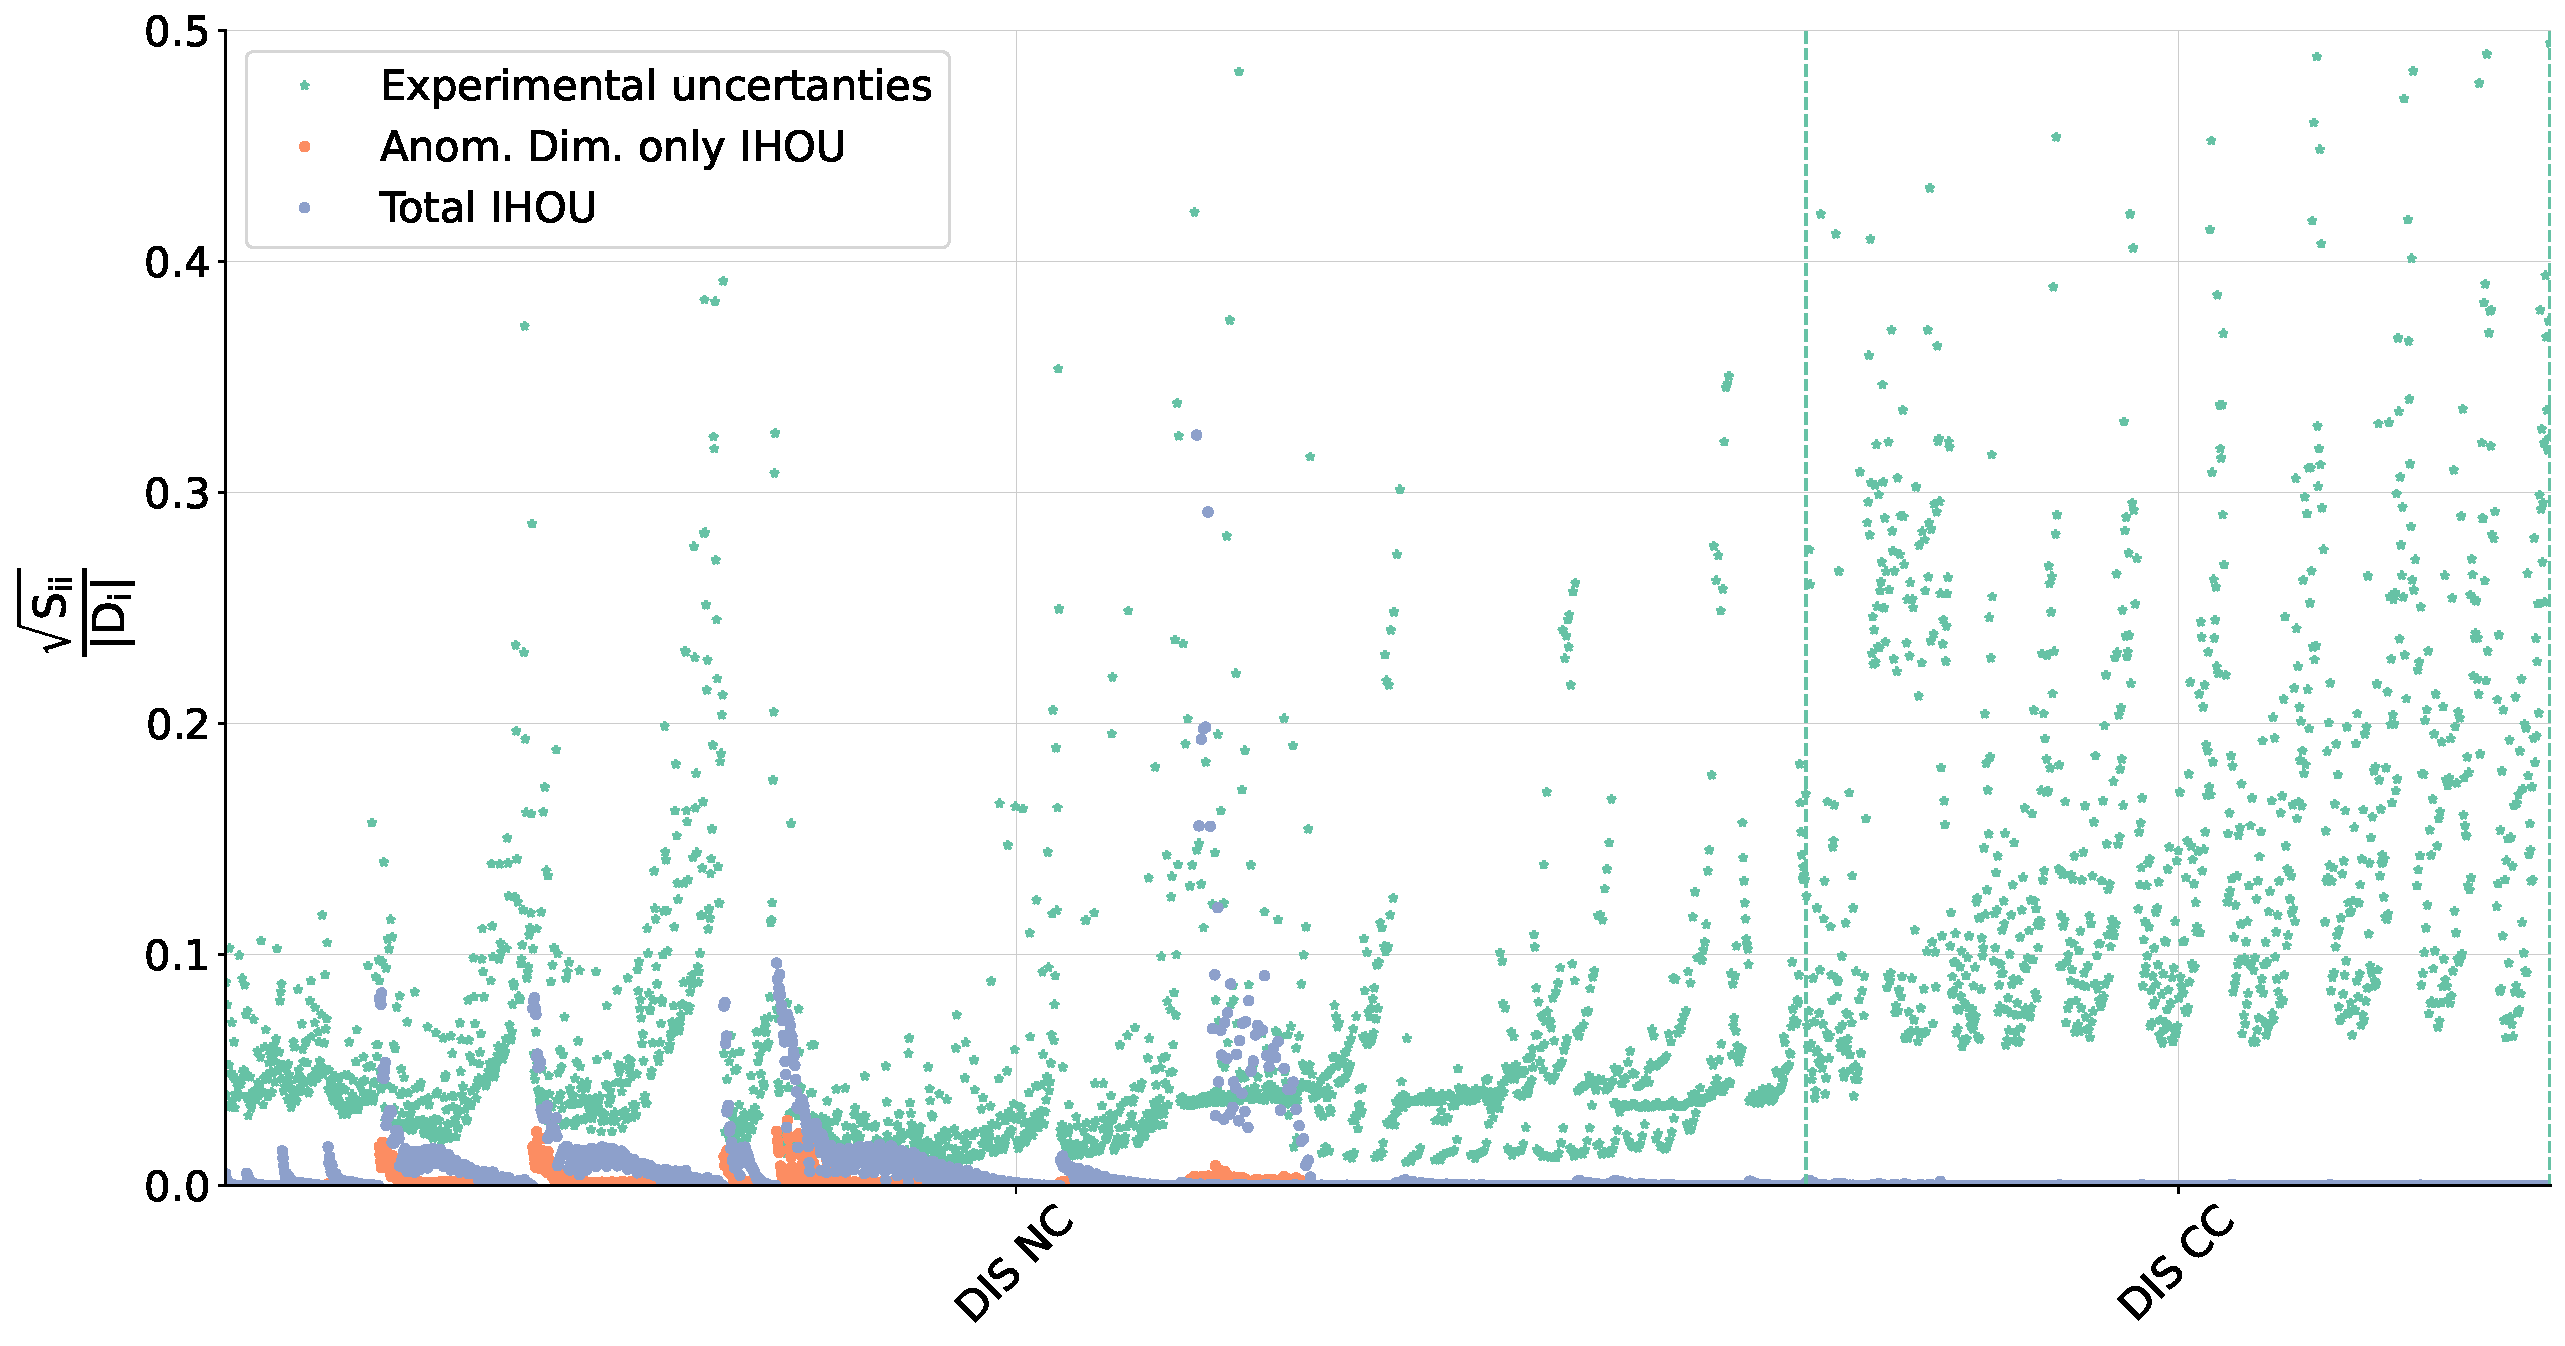
\includegraphics[width=.9\textwidth]{figures/diag_cov_dis_ihou.pdf}
        \caption*{IHOU have a large effect on small-$x$, low-$Q$ DIS data
        }
      \end{figure}
    \end{column}
    \begin{column}{0.49\textwidth}
      \begin{figure}[!t]
        \centering
        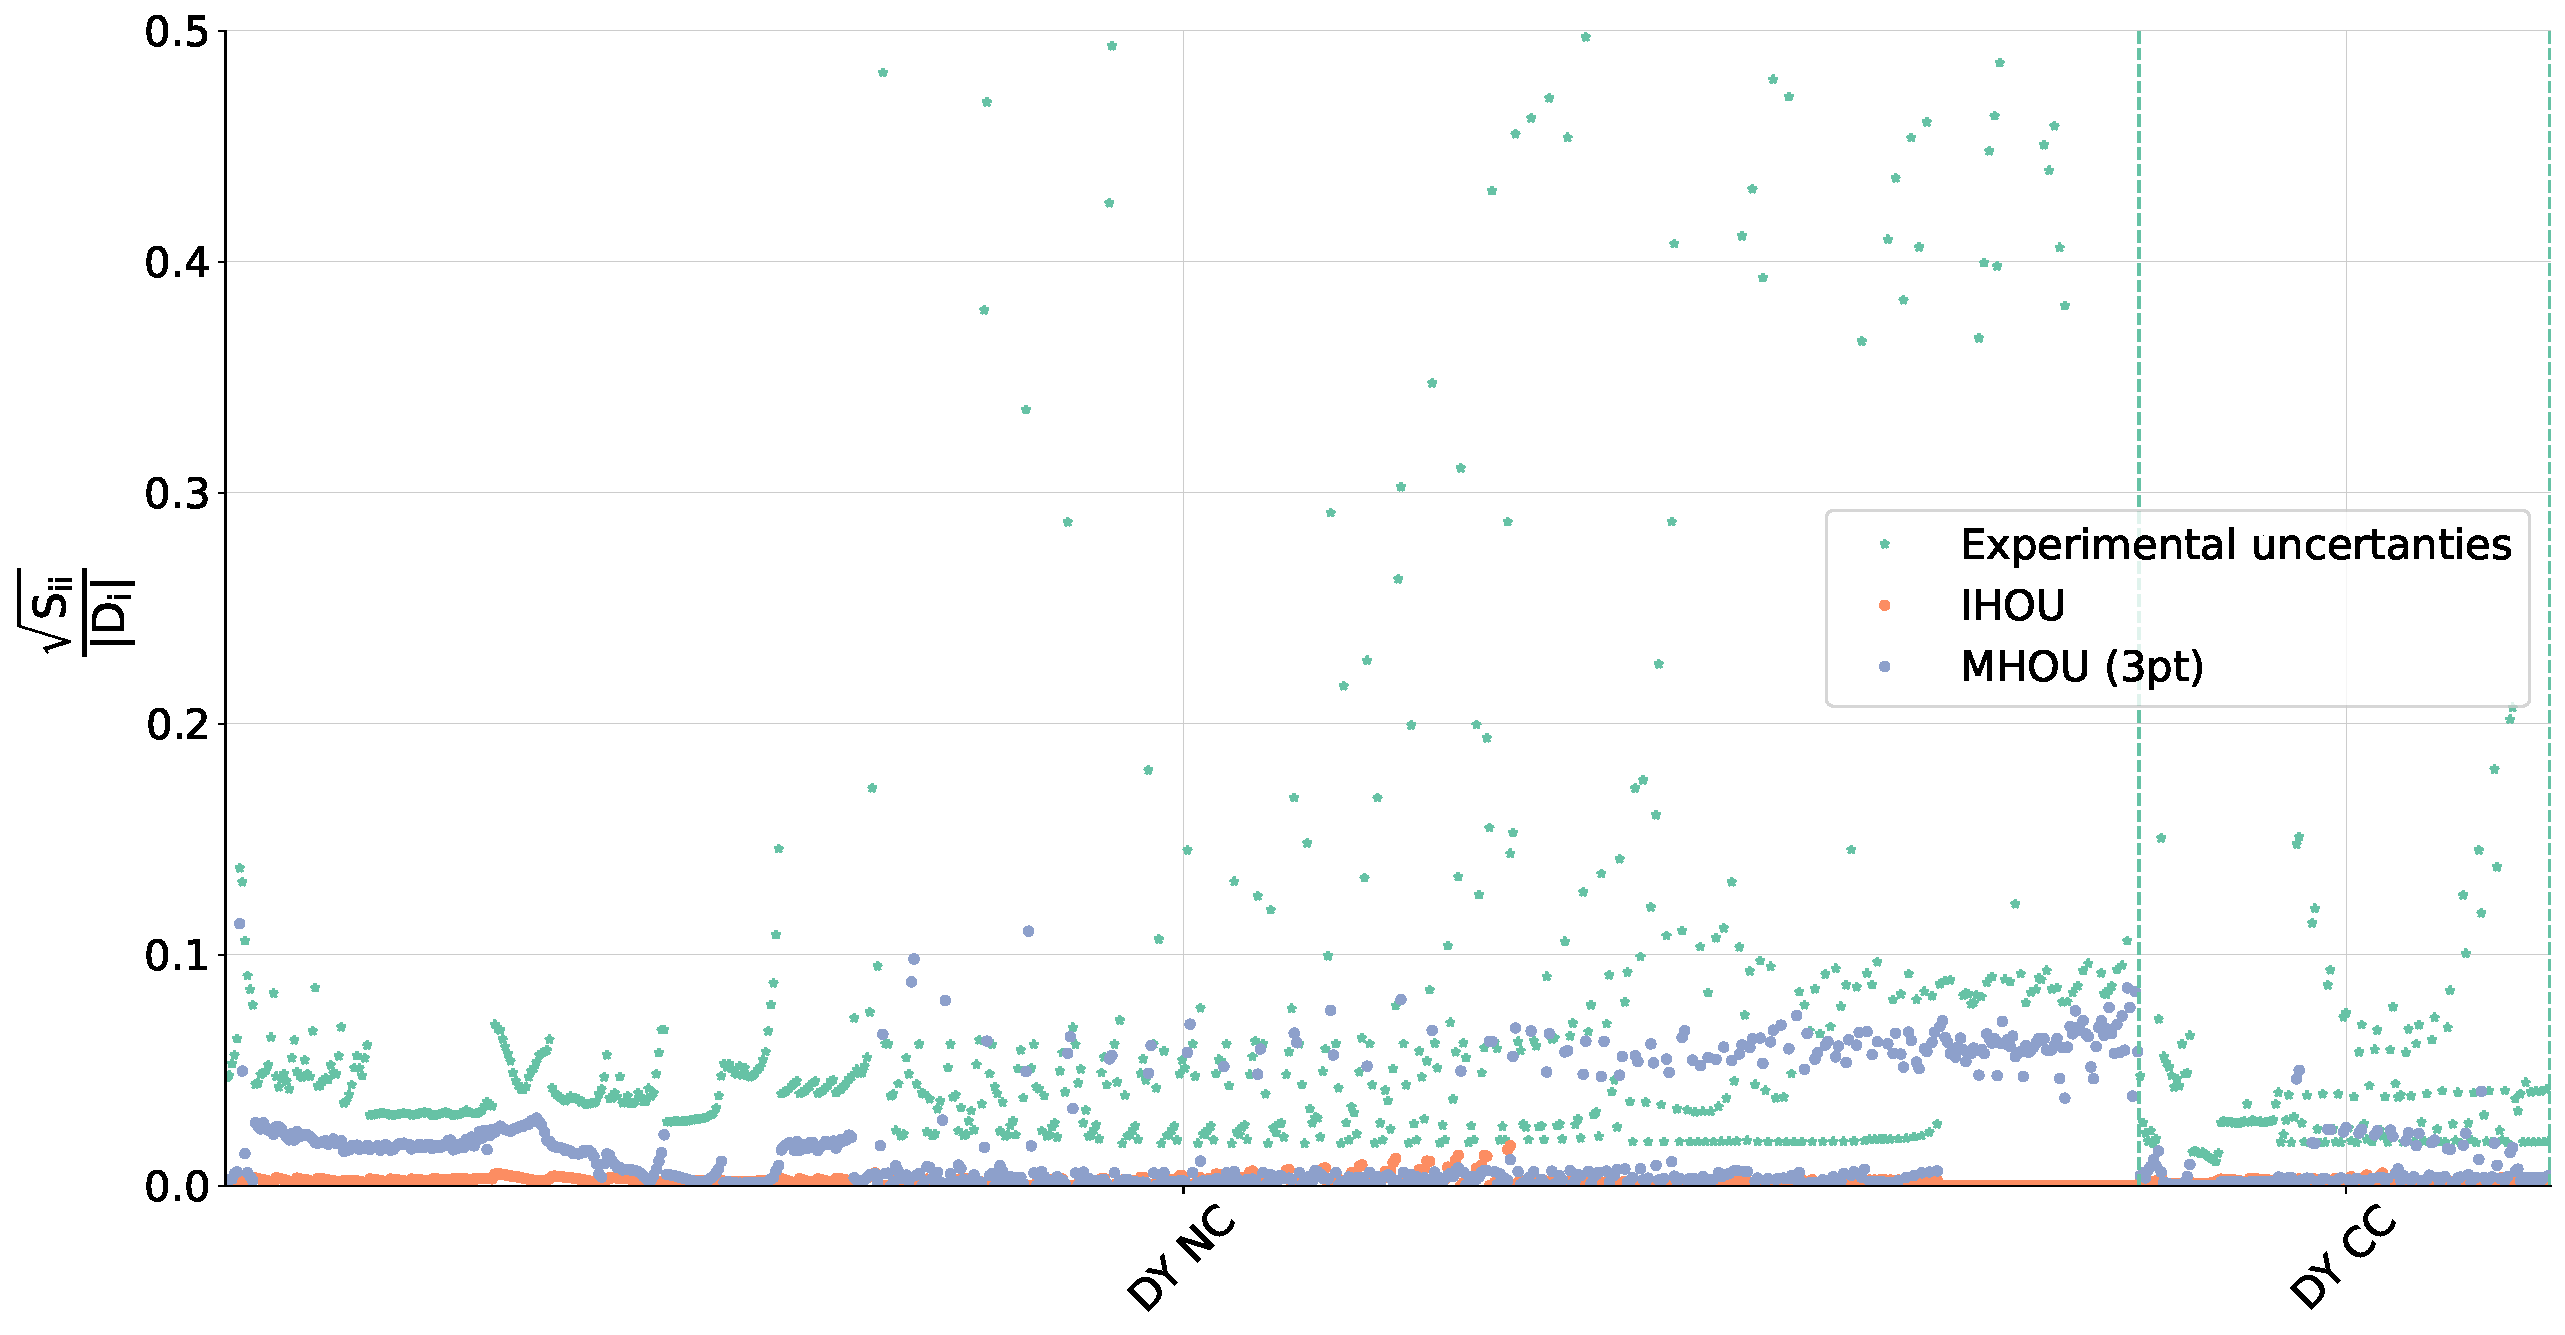
\includegraphics[width=.9\textwidth]{figures/diag_cov_dy_ihou_3pt_mhou.pdf}
        \caption*{NNLO MHOU included where N3LO not available \\
          MHOU can similar magnitude as the experimental uncertainty
        }
      \end{figure}
    \end{column}
  \end{columns}


\end{frame}

% \begin{frame}{Magnitude of theory uncertainties}
% % show that for certain processes th unc is of same size as exp unc.
% \end{frame}

% ============================================================================

\begin{frame}{Impact of MHOUs at N3LO}
  \begin{figure}[!t]
    \centering
    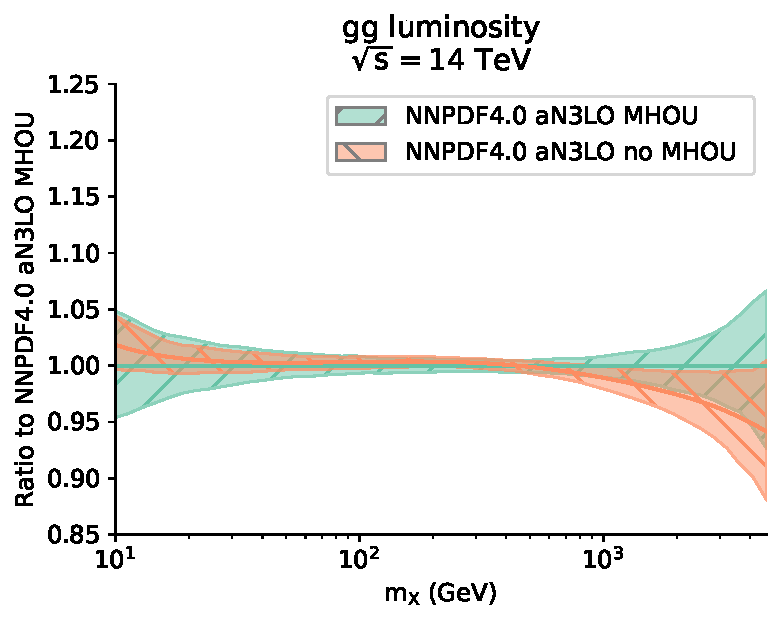
\includegraphics[width=0.45\textwidth]{figures/gg_plot_lumi1d.pdf}
    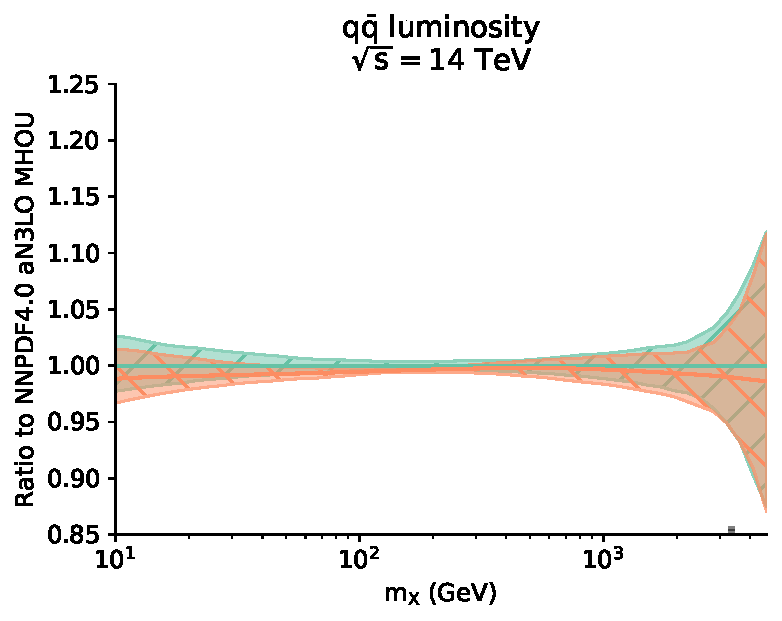
\includegraphics[width=0.45\textwidth]{figures/qqbar_plot_lumi1d.pdf}
  \end{figure}
  \begin{itemize}
    \item Non-negligible impact of MHOUs even at N3LO
    \item[$\Rightarrow$] reason to include exact N3LO calculations for hadronic processes
  \end{itemize}
\end{frame}


% \begin{frame}{Comparison to MSHT20}
%   \begin{figure}[!t]
%     \centering
%     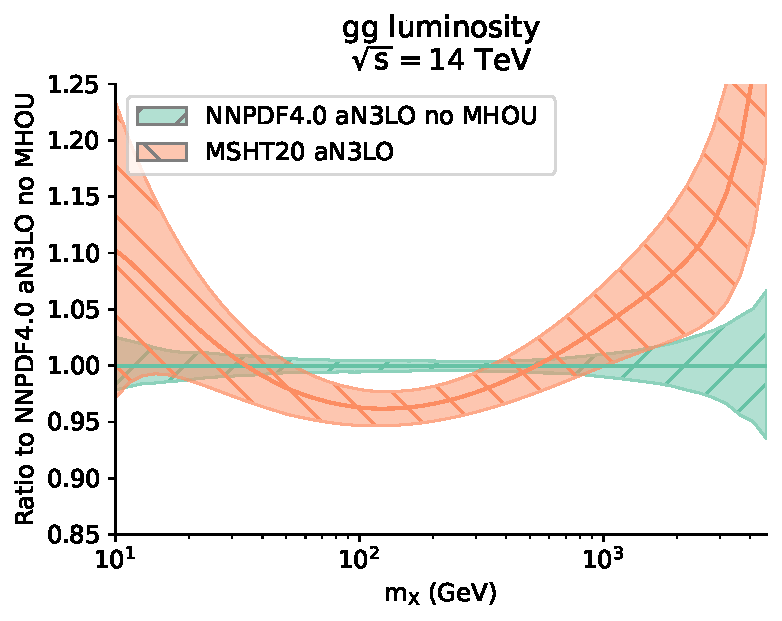
\includegraphics[width=0.45\textwidth]{figures/gg_plot_lumi1d_msht20.pdf}
%     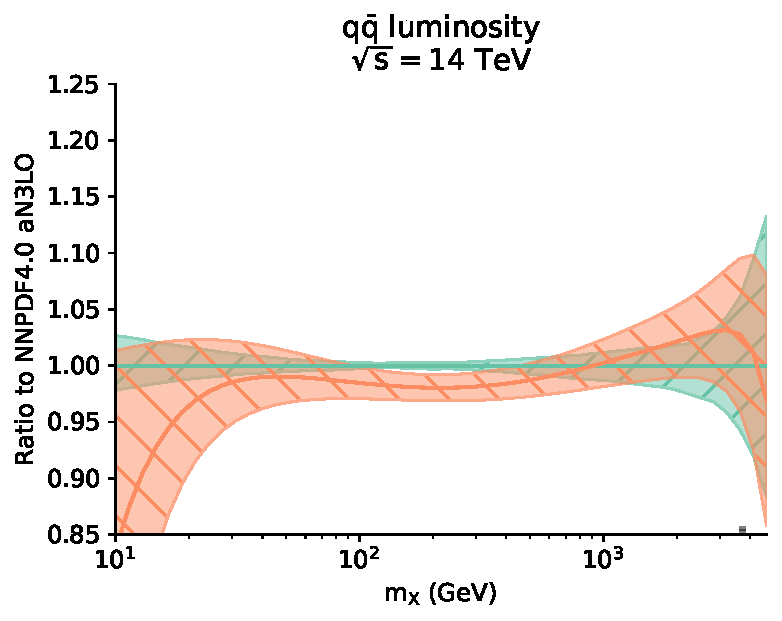
\includegraphics[width=0.45\textwidth]{figures/qqbar_plot_lumi1d_msht20.pdf}
%   \end{figure}
%   \begin{itemize}
%     \item Good agreement with MSHT20 for the quark luminosities
%     \item Also for gluon luminosities, except around the Higgs mass and high-mass
%     \item Similar data but different methodology (including splitting function parametrization)
%   \end{itemize}
% \end{frame}



\end{document}





